\documentclass{standalone}
\usepackage{tikz}
\usetikzlibrary{patterns, positioning}
\usepackage[sfdefault]{ClearSans} %% option 'sfdefault' activates Clear Sans as the default text font
\usepackage[T1]{fontenc}

\begin{document}
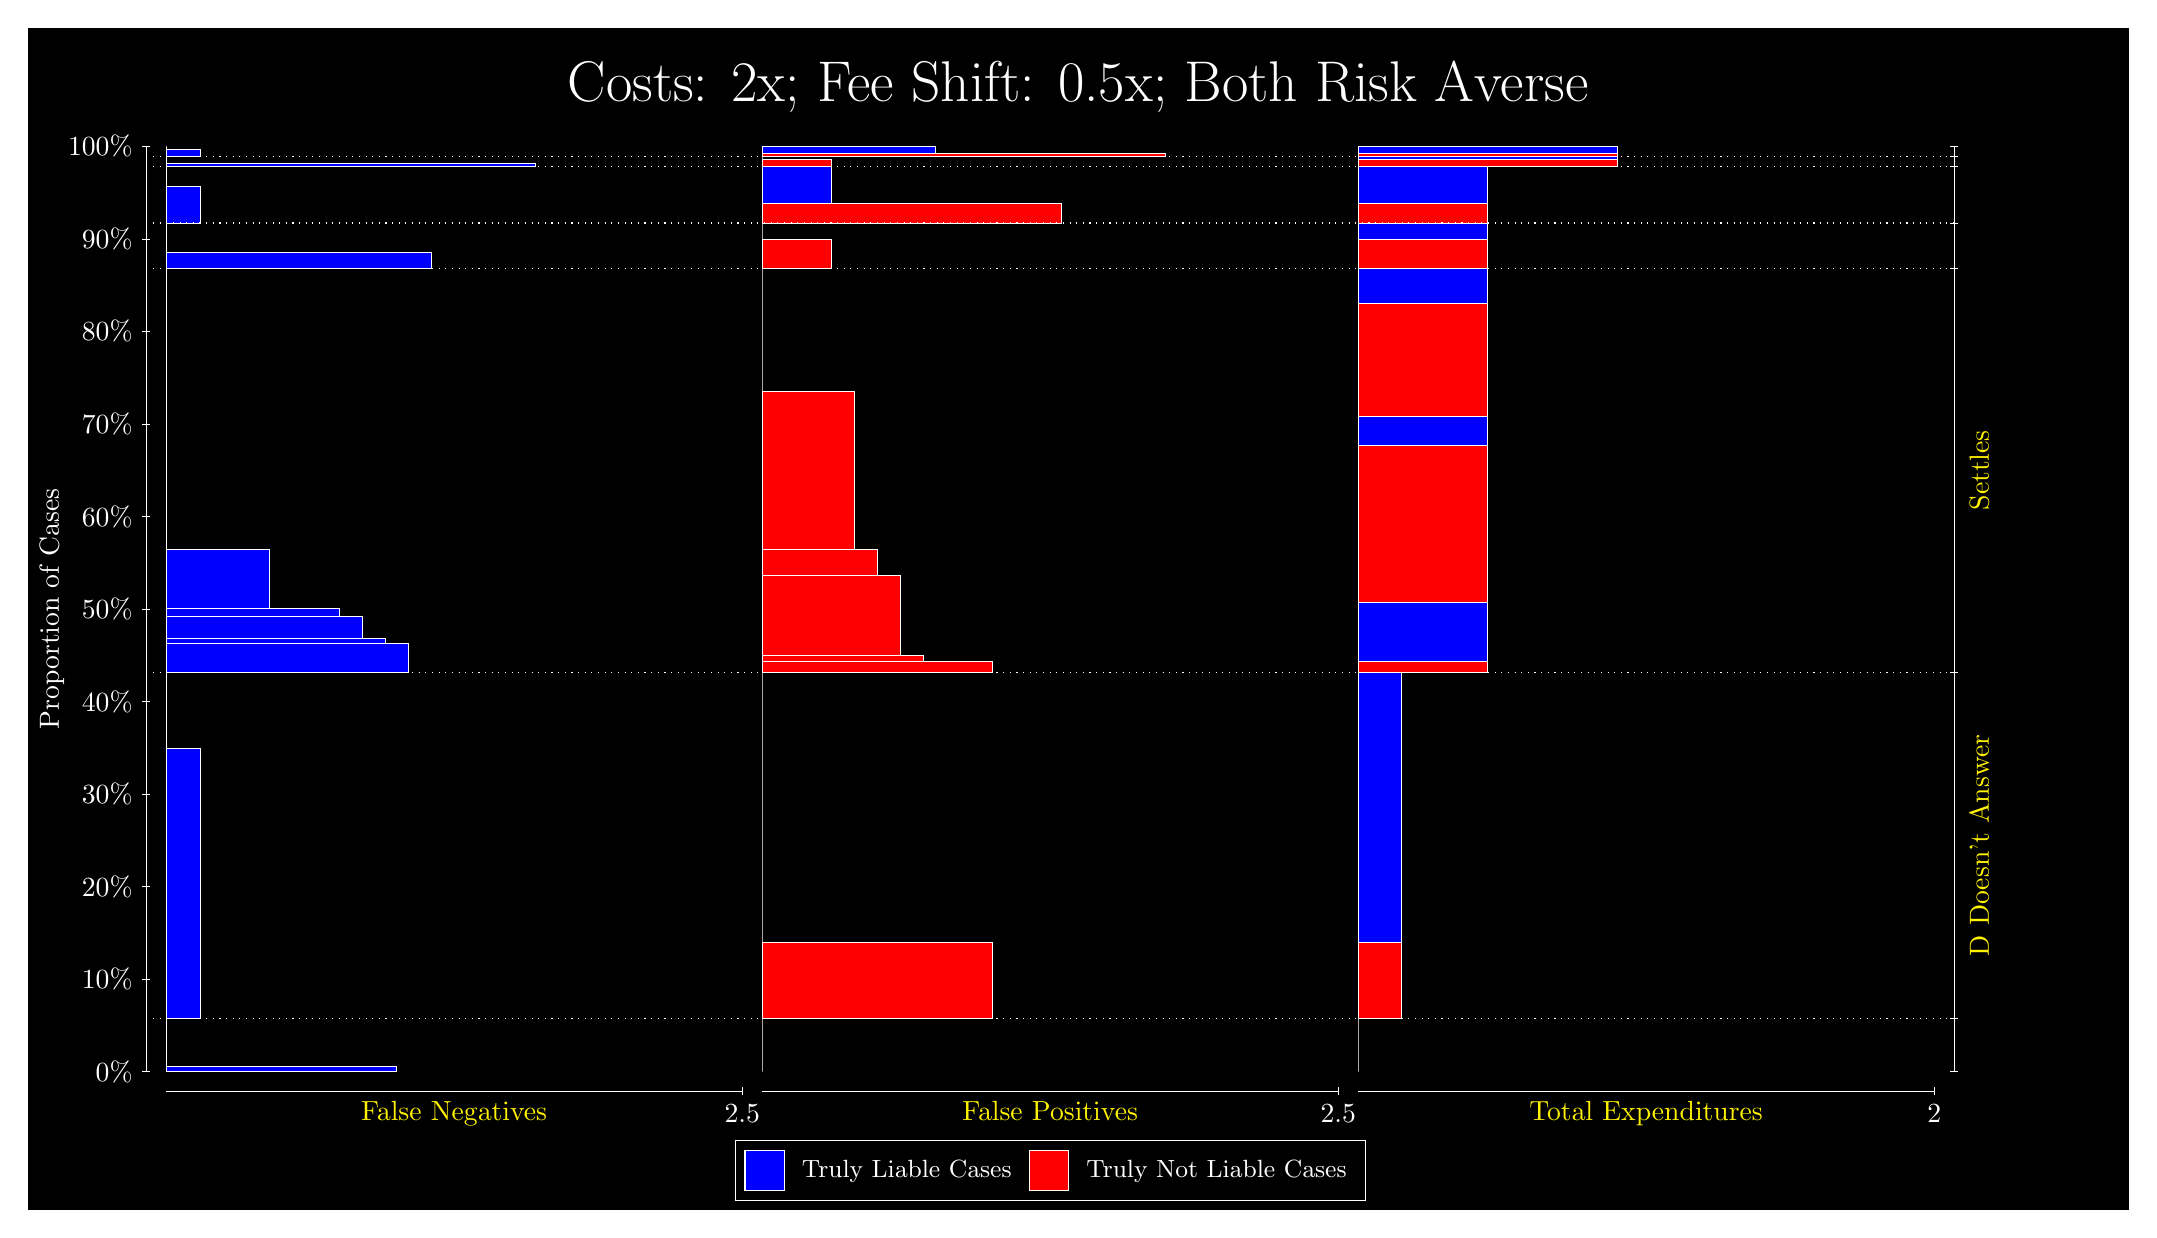
\begin{tikzpicture}
\draw[fill=black] (0,0) rectangle (26.667,15);
\draw[text=white] (0,13.5) rectangle (26.667,15) node[midway] {\huge Costs: 2x; Fee Shift: 0.5x; Both Risk Averse};
\draw[white, very thin] (1.5,1.75) -- (1.5,13.5);
\node[rotate=90, text=white, anchor=center] at (0.3, 7.625) {Proportion of Cases};
\draw[white, very thin] (1.45,1.75) -- (1.55,1.75);
\node[text=white, anchor=east] at (1.45, 1.75) {0\%};
\draw[white, very thin] (1.45,2.925) -- (1.55,2.925);
\node[text=white, anchor=east] at (1.45, 2.925) {10\%};
\draw[white, very thin] (1.45,4.1) -- (1.55,4.1);
\node[text=white, anchor=east] at (1.45, 4.1) {20\%};
\draw[white, very thin] (1.45,5.275) -- (1.55,5.275);
\node[text=white, anchor=east] at (1.45, 5.275) {30\%};
\draw[white, very thin] (1.45,6.45) -- (1.55,6.45);
\node[text=white, anchor=east] at (1.45, 6.45) {40\%};
\draw[white, very thin] (1.45,7.625) -- (1.55,7.625);
\node[text=white, anchor=east] at (1.45, 7.625) {50\%};
\draw[white, very thin] (1.45,8.8) -- (1.55,8.8);
\node[text=white, anchor=east] at (1.45, 8.8) {60\%};
\draw[white, very thin] (1.45,9.975) -- (1.55,9.975);
\node[text=white, anchor=east] at (1.45, 9.975) {70\%};
\draw[white, very thin] (1.45,11.15) -- (1.55,11.15);
\node[text=white, anchor=east] at (1.45, 11.15) {80\%};
\draw[white, very thin] (1.45,12.325) -- (1.55,12.325);
\node[text=white, anchor=east] at (1.45, 12.325) {90\%};
\draw[white, very thin] (1.45,13.5) -- (1.55,13.5);
\node[text=white, anchor=east] at (1.45, 13.5) {100\%};

\draw[white, very thin] (24.457,1.75) -- (24.457,13.5);
\draw[white, very thin] (24.407,1.75) -- (24.507,1.75);
\node[anchor=west] at (24.407, 1.75) {};
\draw[white, very thin] (24.407,2.4242) -- (24.507,2.4242);
\node[anchor=west] at (24.407, 2.4242) {};
\draw[white, very thin] (24.407,6.8207) -- (24.507,6.8207);
\node[anchor=west] at (24.407, 6.8207) {};
\draw[white, very thin] (24.407,11.951) -- (24.507,11.951);
\node[anchor=west] at (24.407, 11.951) {};
\draw[white, very thin] (24.407,12.526) -- (24.507,12.526);
\node[anchor=west] at (24.407, 12.526) {};
\draw[white, very thin] (24.407,13.249) -- (24.507,13.249);
\node[anchor=west] at (24.407, 13.249) {};
\draw[white, very thin] (24.407,13.371) -- (24.507,13.371);
\node[anchor=west] at (24.407, 13.371) {};
\draw[white, very thin] (24.407,13.5) -- (24.507,13.5);
\node[anchor=west] at (24.407, 13.5) {};

\draw[white, very thin, fill=blue] (1.75,1.75) rectangle (4.6775,1.8209);
\draw[white, very thin, fill=red] (1.75,1.8209) rectangle (1.75,2.4242);
\draw[white, very thin, fill=blue] (1.75,2.4242) rectangle (2.1891,5.8575);
\draw[white, very thin, fill=red] (1.75,5.8575) rectangle (1.75,6.8207);
\draw[white, very thin, fill=blue] (1.75,6.8207) rectangle (4.8239,7.1848);
\draw[white, very thin, fill=blue] (1.75,7.1848) rectangle (4.5312,7.2503);
\draw[white, very thin, fill=blue] (1.75,7.2503) rectangle (4.2384,7.5271);
\draw[white, very thin, fill=blue] (1.75,7.5271) rectangle (3.9457,7.6336);
\draw[white, very thin, fill=blue] (1.75,7.6336) rectangle (3.0674,8.3852);
\draw[white, very thin, fill=red] (1.75,8.3852) rectangle (1.75,11.951);
\draw[white, very thin, fill=blue] (1.75,11.951) rectangle (5.1167,12.158);
\draw[white, very thin, fill=red] (1.75,12.158) rectangle (1.75,12.526);
\draw[white, very thin, fill=blue] (1.75,12.526) rectangle (2.1891,12.996);
\draw[white, very thin, fill=red] (1.75,12.996) rectangle (1.75,13.249);
\draw[white, very thin, fill=blue] (1.75,13.249) rectangle (6.4341,13.289);
\draw[white, very thin, fill=red] (1.75,13.289) rectangle (1.75,13.371);
\draw[white, very thin, fill=blue] (1.75,13.371) rectangle (2.1891,13.46);
\draw[white, very thin, fill=red] (1.75,13.46) rectangle (1.75,13.5);
\draw[white, very thin, fill=red] (9.3189,1.75) rectangle (9.3189,2.3533);
\draw[white, very thin, fill=blue] (9.3189,2.3533) rectangle (9.3189,2.4242);
\draw[white, very thin, fill=red] (9.3189,2.4242) rectangle (12.246,3.3875);
\draw[white, very thin, fill=blue] (9.3189,3.3875) rectangle (9.3189,6.8207);
\draw[white, very thin, fill=red] (9.3189,6.8207) rectangle (12.246,6.9554);
\draw[white, very thin, fill=red] (9.3189,6.9554) rectangle (11.368,7.0413);
\draw[white, very thin, fill=red] (9.3189,7.0413) rectangle (11.075,8.0486);
\draw[white, very thin, fill=red] (9.3189,8.0486) rectangle (10.783,8.3883);
\draw[white, very thin, fill=red] (9.3189,8.3883) rectangle (10.49,10.386);
\draw[white, very thin, fill=blue] (9.3189,10.386) rectangle (9.3189,11.951);
\draw[white, very thin, fill=red] (9.3189,11.951) rectangle (10.197,12.319);
\draw[white, very thin, fill=blue] (9.3189,12.319) rectangle (9.3189,12.526);
\draw[white, very thin, fill=red] (9.3189,12.526) rectangle (13.125,12.778);
\draw[white, very thin, fill=blue] (9.3189,12.778) rectangle (10.197,13.249);
\draw[white, very thin, fill=red] (9.3189,13.249) rectangle (10.197,13.331);
\draw[white, very thin, fill=blue] (9.3189,13.331) rectangle (9.3189,13.371);
\draw[white, very thin, fill=red] (9.3189,13.371) rectangle (14.442,13.411);
\draw[white, very thin, fill=blue] (9.3189,13.411) rectangle (11.515,13.5);
\draw[white, very thin, fill=red] (16.888,1.75) rectangle (16.888,2.3533);
\draw[white, very thin, fill=blue] (16.888,2.3533) rectangle (16.888,2.4242);
\draw[white, very thin, fill=red] (16.888,2.4242) rectangle (17.437,3.3875);
\draw[white, very thin, fill=blue] (16.888,3.3875) rectangle (17.437,6.8207);
\draw[white, very thin, fill=red] (16.888,6.8207) rectangle (18.534,6.9554);
\draw[white, very thin, fill=blue] (16.888,6.9554) rectangle (18.534,7.707);
\draw[white, very thin, fill=red] (16.888,7.707) rectangle (18.534,9.705);
\draw[white, very thin, fill=blue] (16.888,9.705) rectangle (18.534,10.069);
\draw[white, very thin, fill=red] (16.888,10.069) rectangle (18.534,11.502);
\draw[white, very thin, fill=blue] (16.888,11.502) rectangle (18.534,11.951);
\draw[white, very thin, fill=red] (16.888,11.951) rectangle (18.534,12.319);
\draw[white, very thin, fill=blue] (16.888,12.319) rectangle (18.534,12.526);
\draw[white, very thin, fill=red] (16.888,12.526) rectangle (18.534,12.778);
\draw[white, very thin, fill=blue] (16.888,12.778) rectangle (18.534,13.249);
\draw[white, very thin, fill=red] (16.888,13.249) rectangle (20.181,13.331);
\draw[white, very thin, fill=blue] (16.888,13.331) rectangle (20.181,13.371);
\draw[white, very thin, fill=red] (16.888,13.371) rectangle (20.181,13.411);
\draw[white, very thin, fill=blue] (16.888,13.411) rectangle (20.181,13.5);
\draw[white, dotted] (1.5,2.4242) -- (24.457,2.4242);
\draw[white, dotted] (1.5,6.8207) -- (24.457,6.8207);
\draw[white, dotted] (1.5,11.951) -- (24.457,11.951);
\draw[white, dotted] (1.5,12.526) -- (24.457,12.526);
\draw[white, dotted] (1.5,13.249) -- (24.457,13.249);
\draw[white, dotted] (1.5,13.371) -- (24.457,13.371);
\draw[white, very thin] (1.75,1.5) -- (9.0689,1.5);
\node[text=yellow, anchor=north] at (5.4094, 1.5) {False Negatives};
\draw[white, very thin] (9.0689,1.45) -- (9.0689,1.55);
\node[text=white, anchor=north] at (9.0689, 1.45) {2.5};

\draw[white, very thin] (9.3189,1.5) -- (16.638,1.5);
\node[text=yellow, anchor=north] at (12.978, 1.5) {False Positives};
\draw[white, very thin] (16.638,1.45) -- (16.638,1.55);
\node[text=white, anchor=north] at (16.638, 1.45) {2.5};

\draw[white, very thin] (16.888,1.5) -- (24.207,1.5);
\node[text=yellow, anchor=north] at (20.547, 1.5) {Total Expenditures};
\draw[white, very thin] (24.207,1.45) -- (24.207,1.55);
\node[text=white, anchor=north] at (24.207, 1.45) {2};


\node[text=yellow, centered, rotate=90] at (24.777, 4.6225) {D Doesn't Answer};
\node[text=yellow, centered, rotate=90] at (24.777, 9.3857) {Settles};





\draw (12.978300999999998,1.5) node[draw=none] (baseCoordinate) {};
\begin{scope}[align=center]
        \matrix[scale=0.5, draw=white, below=0.5cm of baseCoordinate, nodes={draw}, column sep=0.1cm]{
            \node[rectangle, draw, minimum width=0.5cm, minimum height=0.5cm, fill=blue] {}; &
            \node[draw=none, font=\small, text=white] (B) {Truly Liable Cases}; &
            \node[rectangle, draw, minimum width=0.5cm, minimum height=0.5cm, fill=red] {}; &
            \node[draw=none, font=\small, text=white] (B) {Truly Not Liable Cases}; \\
            };
\end{scope}

\end{tikzpicture}
\end{document}